\tcbset{
  myboxstyle/.style={
    boxrule=1pt,
    boxsep=2pt,
    colback=gray!5,
    fontupper=\scriptsize,
    fonttitle=\color{black},
    title=Scene Description Example,
    coltitle=black,
    colframe=black,
    colbacktitle=blue!10,
    breakable
  }
}

\tcbset{
  myjsonbox/.style={
    enhanced,
    colframe=gray!50,
    colback=white,
    fonttitle=\small\color{white},
    boxrule=0.8pt,
    arc=4pt,
    left=4pt,
    right=4pt,
    top=4pt,
    bottom=4pt,
    boxsep=5pt,
    listing only,
    listing options={
      language=json,
      basicstyle=\scriptsize\ttfamily,
      keywordstyle=\color{blue},
      stringstyle=\color{orange!90!black},
      commentstyle=\color{gray},
      morekeywords={true,false,null},
      literate=%
        *{,}{{\textcolor{red}{,}}}{1}%
         {:}{{\textcolor{red}{:}}}{1}%
         {\{}{{\textcolor{red}{\{}}}{1}%
         {\}}{{\textcolor{red}{\}}}}{1}%
    },
    breakable,
  }
}

\lstdefinelanguage{json}{
    basicstyle=\ttfamily\footnotesize,
    showstringspaces=false,
    breaklines=true,
    breakatwhitespace=true,
    morestring=[b]",
    stringstyle=\color{orange!90!black},
    morecomment=[s]{/*}{*/},
    commentstyle=\color{gray},
    morekeywords={true,false,null},
    keywordstyle=\color{blue},
    literate=%
      *{,}{{\textcolor{red}{,}}}{1}%
       {:}{{\textcolor{red}{:}}}{1}%
       {\{}{{\textcolor{red}{\{}}}{1}%
       {\}}{{\textcolor{red}{\}}}}{1}%
}




\begin{tcolorbox}[myboxstyle]

\begin{center}
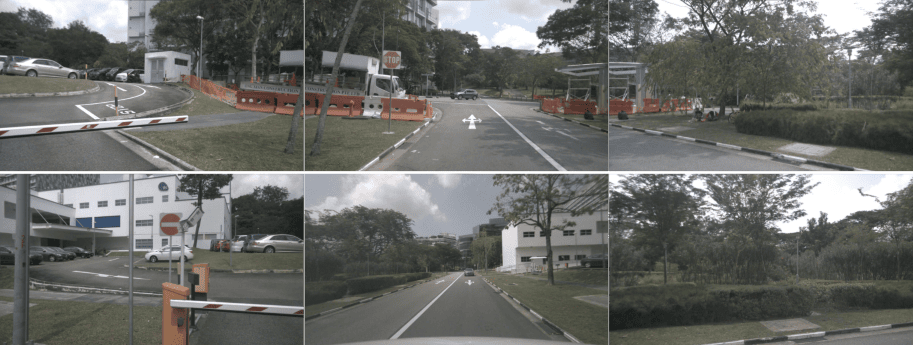
\includegraphics[width=0.9\linewidth]{src/description_exp2.png}
\end{center}

\vspace{1ex}

\noindent\textbf{\textcolor{purple}{Scene Style:}}
\begin{itemize}[leftmargin=15pt, itemsep=2pt]
    \item \textcolor{blue}{Time of the day}: bright daytime with clear shadows, indicating direct sunlight and good visibility
    \item \textcolor{blue}{Weather}: sunny with partly cloudy skies; no signs of precipitation or poor visibility
    \item \textcolor{blue}{Surrounding environment}: suburban campus or business park-like area with a mix of roadways, pedestrian paths, and landscaped
    \item \textcolor{blue}{Road condition}: smooth asphalt with a gentle curve transitioning into a straight segment




\end{itemize}

\noindent\textbf{\textcolor{purple}{Foreground Objects:}}
\begin{itemize}[leftmargin=15pt, itemsep=2pt]
  \item \textcolor{blue}{Barriers (construction zone)}: bright orange modular barriers clearly indicating a temporarily restricted area
  \item \textcolor{blue}{Truck (construction zone)}: a white construction truck with visible text parked adjacent to the barriers
  \item \textcolor{blue}{Stop sign (construction zone)}: standard red octagonal stop sign mounted on a metallic pole, reinforcing right-of-way rules
  \item \textcolor{blue}{Entrance barrier}:  red and white striped boom barrier at two vehicle access points, indicating controlled entry
  \item \textcolor{blue}{Cars}: silver sedan (parked at curve near the booth); black sedan (alongside silver); dark-colored sedan (moving towards camera, on central lane); red and silver vehicles (visible in side/rear view near building and behind the no-entry sign)
  \item \textcolor{blue}{Seated pedestrian}: a person is resting on the grassy area near the right side of the road, shaded by trees
\end{itemize}

\noindent\textbf{\textcolor{purple}{Background Elements:}}
\begin{itemize}[leftmargin=15pt, itemsep=2pt]
  \item \textcolor{blue}{Road}: dual-lane road with center markings and white directional arrows
  \item \textcolor{blue}{Sidewalk}: paved pathways flanked by grass and shrubs on both sides of the road
  \item \textcolor{blue}{Buildings}: main visible structure is a multi-story white facility with large windows and blue signage
  \item \textcolor{blue}{Vegetation}: tall green trees forming canopy along both sides of the road, sculpted bushes reinforce the planned landscape design
  \item \textcolor{blue}{Car Parking}: clearly delineated lot visible on the left, populated with multiple parked cars
  \item \textcolor{blue}{Traffic Signage}: a “No Entry” (red circle with horizontal white bar) sign prominently displayed at an access control gate
\end{itemize}


\noindent\textbf{\textcolor{purple}{Scene-Graph Layout:}}
\begin{center}
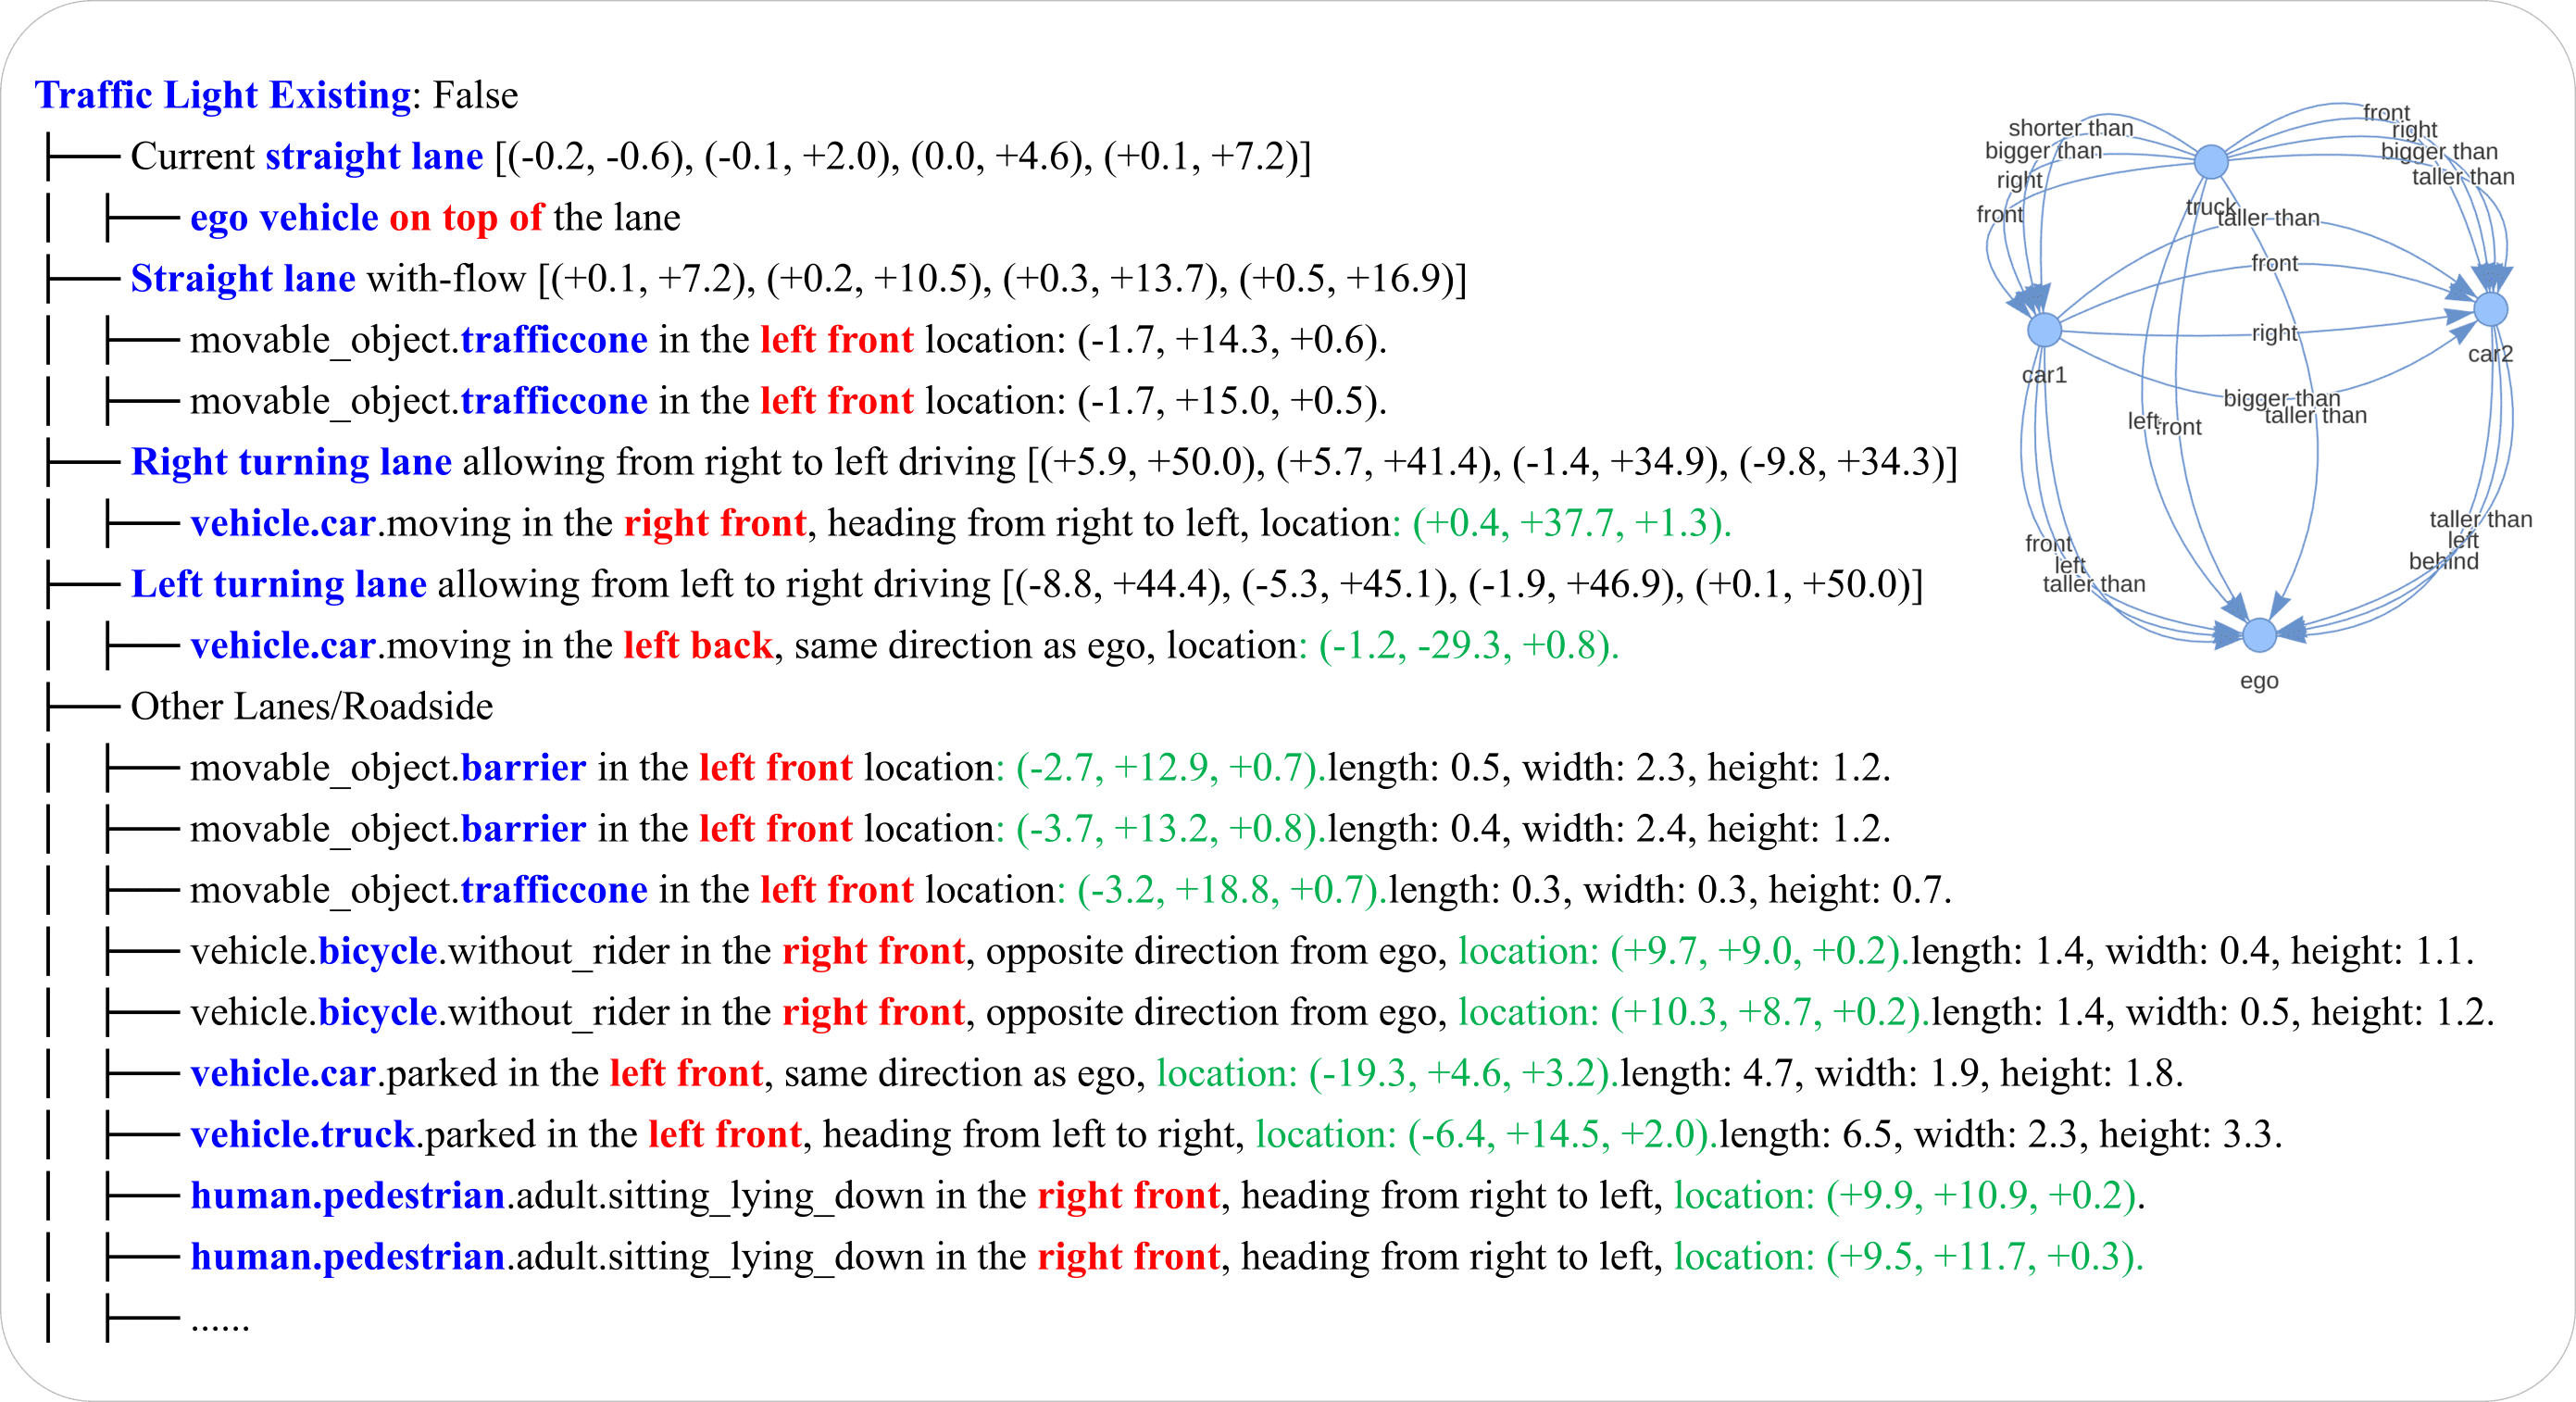
\includegraphics[width=0.98\linewidth]{src/layout2.png}
\end{center}


\noindent\textbf{\textcolor{purple}{Abstract Description:}}
\begin{itemize}[leftmargin=15pt, itemsep=2pt]
  \item \textcolor{gray!10!black}{The scene shows a sunny day in a suburban area with a mix of urban infrastructure and greenery. The road curves slightly before straightening out, with construction barriers and a stop sign indicating ongoing work. Several cars are parked along the roadside, while others are in motion. A pedestrian is seated on the grass near the right-rear view, and there are trees and buildings in the background. The road appears well-maintained, with clear lane markings and a mix of open spaces and developed areas.}
\end{itemize}

\end{tcolorbox}
